\documentclass[a4paper]{article}

\usepackage{geometry}
\usepackage{bm}
\usepackage{fancyvrb,color,gretl}
%\usepackage{mathpazo}
\usepackage{amsmath}
\usepackage{graphicx}

\setlength{\parskip}{1ex}
\setlength{\parindent}{0pt}

\title{Kalman Filter GUI}
\author{Jack Lucchetti}
\date{\it this facility is work in progress}

\newcommand{\obs}{\ensuremath\mathbf{y}_t}
\newcommand{\obsdist}{\ensuremath\boldsymbol{\varepsilon}_t}
\newcommand{\state}[1]{\ensuremath\boldsymbol{\mu}_{#1}}
\newcommand{\stdist}{\ensuremath\boldsymbol{\eta}_t}
\newcommand{\param}{\ensuremath\boldsymbol{\theta}}

\begin{document}
\maketitle

The goal here is to provide a native GUI hook so as to give some more
visibility to the facilities gretl has available for state space
modelling (\texttt{ksetup()} and friends).

The GUI hook presented here can be used for performing ML estimation of
models of the kind
\begin{eqnarray}
  \label{eq:obs}
  \obs & = & Z \state{t} + \obsdist \\
  \label{eq:state}
  \state{t} & = & T \state{t-1} + R \stdist
\end{eqnarray}
where $V(\obsdist)$ and $V(\stdist)$ are diagonal matrices; in fact,
$\obsdist$ may have zero variance, in which case $\obsdist$ is
identically 0 and the last term of equation (\ref{eq:obs}) is
dropped. The matrix $R$ is useful for cases when the covariance matrix
of the state transition equation is singular.

The system matrices $Z$, $T$ and $R$ are assumed to be known,
so estimation only concerns the variances of $\obsdist$ and $\stdist$.
Clearly, this is a very limited subset of the range of models that
gretl can handle, but it may be of some pedagogical value.

ML estimation is carried out internally using the \texttt{mle}
command, but of course when this is re-done in GTK we may decide use
the BFGS optimizer natively (even though part of this code could
remain in hansl for easier maintenance, like we do with parts of the
\texttt{dbnomics} addon). The only caveat is about parametrization. In
fact, for reasons of numerical performance, it is convenient to have
the choice of representing variances as transformations of the BFGS
parameters in one of the three following ways:

\begin{description}
\item[Absolute value] maximization is performed on the variances:
  $\sigma^2 = |\theta|$
\item[Square] maximization is performed on the standard deviations:
  $\sigma^2 = \theta^2$
\item[Exponential] maximization is performed on the log standard deviations:
  $\sigma^2 = \exp(2 \cdot \theta)$
\end{description}

Normally, this choice should make no difference for well-behaved
data. In any case, the function reports the estimates of the standard
errors whatever the parametrization type.

Once the parameters are estimated the user has the choice of
performing the smoothing of the states.

\begin{figure}[htbp]
  \centering
  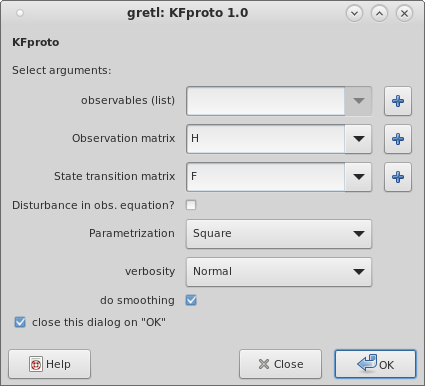
\includegraphics[scale=0.5]{GUIScreenshot.png}
  \caption{GUI hook for state space models}
  \label{fig:GUI}
\end{figure}

The GUI hook is shown in figure \ref{fig:GUI}: the ``observables'' box
is used for specifying a list of series for $\obs$. The next two boxes
handle the $Z$ and $T$ matrices, respectively. These can be
pre-existing matrices or created ``on the fly'' using the GUI facility
we have for that. The remaining GUI elements should hopefully be
self-explanatory.

The function returns a bundle which includes a sub-bundle called
\texttt{kmod} with all the state-space internals; a matrix called
\texttt{state} holding the estimated states; and matrices
\texttt{coeff} and \texttt{vcv} holding respectively, the coefficients
and standard obtained via ML estimation.

\section*{Example: Random walk plus noise}

The model here is
\[
  y_t = \mu_t + \varepsilon_t \qquad \mu_t = \mu_{t-1} + \eta_t
\]
so that $Z = T = 1$. The following script simulates the DGP above
with $V(\varepsilon) = 1$ and $V(\eta) = 1/8$.

\begin{code}
clear
set verbose off
include KFgui.gfn

set seed 280921

nulldata 256
setobs 1 1 --special

# example 1: random walk plus noise

series m = cum(normal() * 0.25)
series y = m + normal()
Z = {1}
T = {1}
do_smooth = 1
paramtype = 2
b = KFproto (y, Z, T, 1, paramtype, 1, do_smooth)
series mhat = b.state
gnuplot m mhat --time-series --with-lines --output=display
\end{code}

which returns the output below and the picture shown in Figure
\ref{fig:state}

\begin{code}
Observation equation

             coefficient   std. error     z     p-value 
  ------------------------------------------------------
  stdev[1]    0.939311     0.0496287    18.93   6.86e-80 ***


State transition equation

             coefficient   std. error     z     p-value 
  ------------------------------------------------------
  stdev[1]    0.274650     0.0488920    5.617   1.94e-08 ***

  Log-likelihood = -388.946
\end{code}


\begin{figure}[hb]
  \centering
  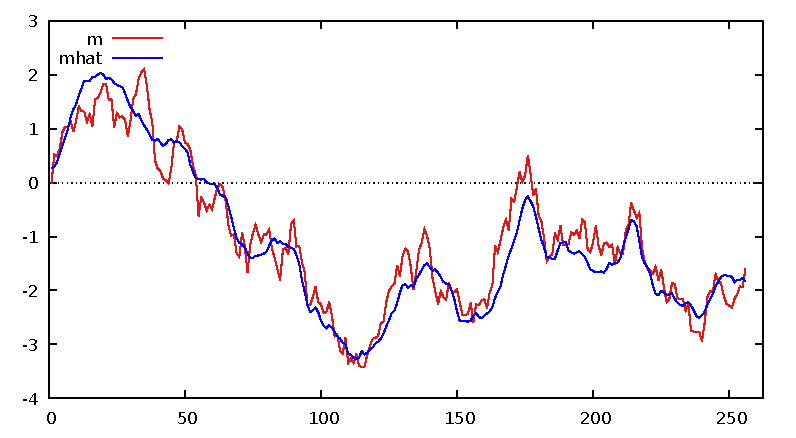
\includegraphics[scale=0.7]{state}
  \caption{Estimated state}\label{fig:state}
\end{figure}

\section*{Example: Random walk plus noise plus seasonal}

The model here is
\[
  y_t = \mu_t + s_t + \varepsilon_t,
\]
where $\mu_t = \mu_{t-1} + \eta_{1,t}$, like in the previous example
and $s_t$ is a seasonal component, implicitly defined by the property
\[
  s_t = -\sum_{j=1}^{S-1} s_{t-i} + \eta_{2,t},
\]
$S$ being the number of subperiods. For example, with quarterly data
the system matrices would be
\[
  Z = \begin{bmatrix}  1 & 1 & 0 & 0  \end{bmatrix}
  \quad
  T = \begin{bmatrix}
    1 & 0 & 0 & 0 \\
    0 & -1 & -1 & -1 \\
    0 & 1 & 0 & 0 \\
    0 & 0 & 1 & 0
  \end{bmatrix}
  \quad
  R = \begin{bmatrix}  1 & 0 \\ 0 & 1 \\ 0 & 0 \\ 0 & 0   \end{bmatrix}
\]

The following script applies this model to one of the series in the
gretl examnple dataset \texttt{data9-3.gdt}:

\begin{code}
set verbose off
include KFgui.gfn
open data9-3
y = log(reskwh)

Z = ones(2,1) | zeros(2,1)
SeasMat = -ones(1,3) | I(2,3)
T = diagcat(1, SeasMat)
R = I(2) | zeros(2,2)

bun = KFgui(y, Z, T, R)

series trend = bun.state[,1]
series seas = bun.state[,2]

scatters y trend seas
\end{code}

which returns the output below and the picture shown in Figure
\ref{fig:rw+seas}

\begin{code}

Observation equation

             coefficient   std. error     z     p-value
  -----------------------------------------------------
  stdev[1]    0.0173633    0.00448117   3.875   0.0001  ***


State transition equation

             coefficient   std. error     z     p-value 
  ------------------------------------------------------
  stdev[1]   0.0269790     0.00409457   6.589   4.43e-11 ***
  stdev[2]   0.00648082    0.00202576   3.199   0.0014   ***

  Log-likelihood = 121.33
\end{code}

\begin{figure}[hb]
  \centering
  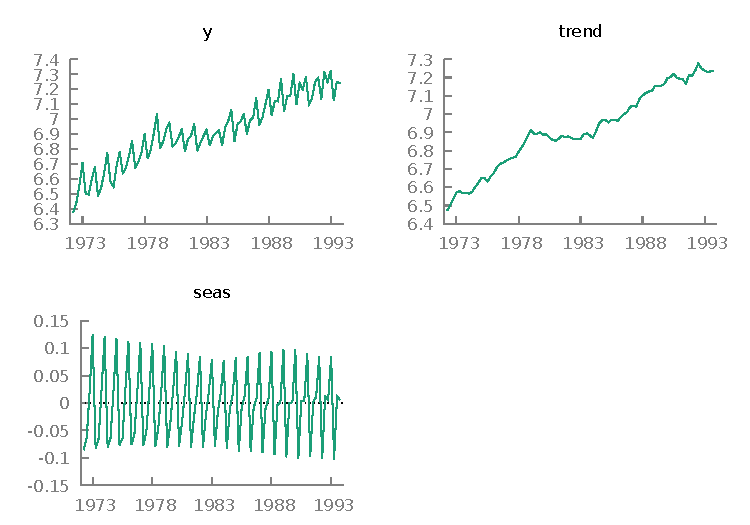
\includegraphics[scale=0.7]{rw+seas}
  \caption{Estimated state}\label{fig:rw+seas}
\end{figure}


\end{document}

%%% Local Variables:
%%% mode: latex
%%% TeX-master: t
%%% End:
